\begin{center}
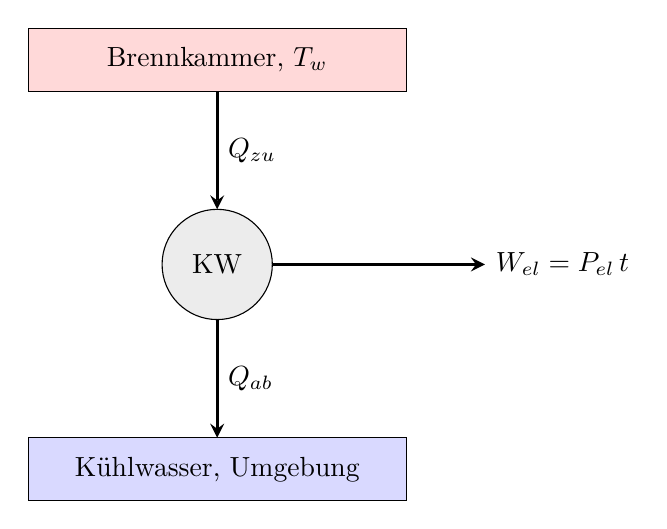
\begin{tikzpicture}[>=stealth]
 \draw[fill=red!15] (-2.4,2.2) rectangle (2.4,3.0);
 \node at (0,2.6) {Brennkammer, $T_\text{w}$};
 \draw[fill=gray!15] (0,0) circle (0.7);
 \node at (0,0) {KW};
 \draw[fill=blue!15] (-2.4,-2.2) rectangle (2.4,-3.0);
 \node at (0,-2.6) {Kühlwasser, Umgebung};
 \draw[->, very thick] (0,2.2) -- (0,0.7) node[midway, right] {$Q_\text{zu}$};
 \draw[->, very thick] (0,-0.7) -- (0,-2.2) node[midway, right] {$Q_\text{ab}$};
 \draw[->, very thick] (0.7,0) -- (3.4,0) node[right] {$W_\text{el} = P_\text{el}\,t$};
\end{tikzpicture}
\end{center}

In der Zeit $t$ wird die elektrische Energie $W_\text{el} = P_\text{el}\,t$ produziert. Dafür muss die Wärme $Q_\text{zu} = W_\text{el}/\eta$ zugeführt werden. Der Rest ist Abwärme (Energieerhaltung):
\begin{align}
 Q_\text{ab} &= Q_\text{zu} - W_\text{el} = \frac{P_\text{el}\,t}{\eta} - P_\text{el}\,t = \QabF \\
   &= \Pel\cdot\tS\cdot\frac{1-\etKO}{\etKO} \\
   &= \Qab \approx \result{\QabP{12}{2}}
\end{align}
Die Abwärme ist fast doppelt so gross wie die produzierte elektrische Energie.
